\section{Graphes planaires}

% TODO Alexis, please merge BEGIN->MIDDLE and MIDDLE->END

% TODO BEGIN

Un graphe est planaire si il possède une représentation dans le plan dont les arêtes ne se touchent pas, sauf à leurs extrémités.\\

\begin{mytheo}[Conjoncture des quatre couleurs]
Quatre couleurs suffisent toujours pour colorier une carte
\begin{proof}
On suppose qu'en chaque point se rencontrent au maximum trois pays, et que les pays sont d'un seul tenant.\\

\begin{center}
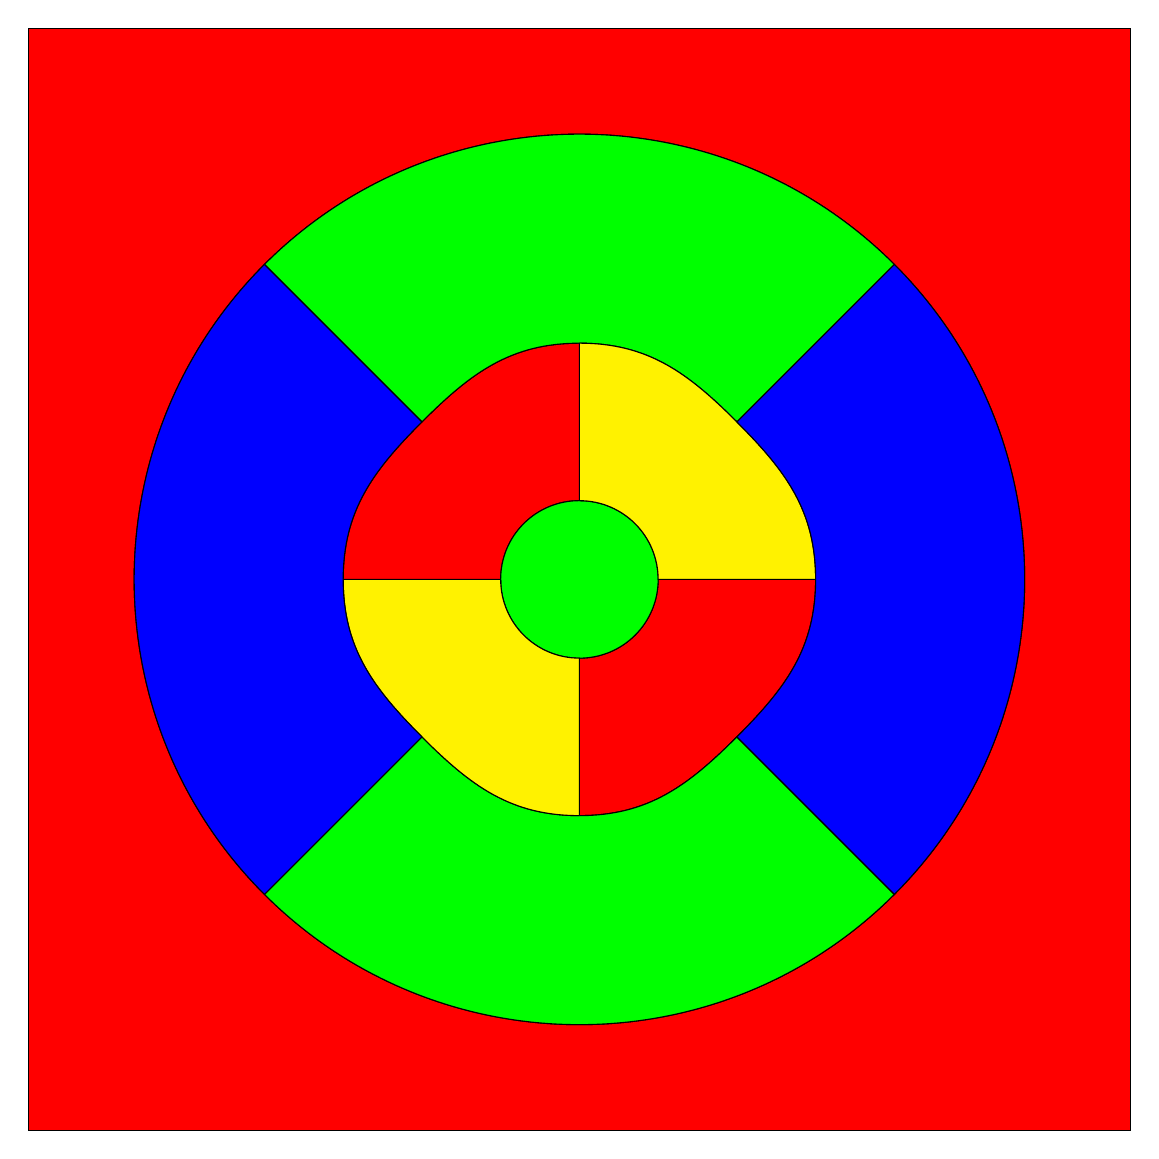
\begin{tikzpicture}
%Outer box
\draw[fill=red] (-3,-3)--(-3,11)--(11,11)--(11,-3)--cycle;
%Outer circle
\draw (0,0) to[out=135,in=-135] (0,8);
\draw (0,8) to[out=45,in=135] (8,8);
\draw (8,8) to[out=-45,in=45] (8,0);
\draw (8,0) to[out=-135,in=-45] (0,0);

%First inner circle
\draw (1,4) to[out=90,in=-135] (2,6);
\draw (2,6) to[out=45,in=-180] (4,7);
\draw (4,7) to[out=0,in=135] (6,6);
\draw (6,6) to[out=-45,in=90] (7,4);
\draw (7,4) to[out=-90,in=45] (6,2);
\draw (6,2) to[out=-135,in=0] (4,1);
\draw (4,1) to[out=-180,in=-45] (2,2);
\draw (2,2) to[out=135,in=-90] (1,4);

%Second inner circle
\draw (3,4) to[out=90,in=-180] (4,5);
\draw (4,5) to[out=0,in=90] (5,4);
\draw (5,4) to[out=-90,in=0] (4,3);
\draw (4,3) to[out=-180,in=-90] (3,4);

%Links from Outer to first inner
\draw (0,0)--(2,2);
\draw (0,8)--(2,6);
\draw (8,8)--(6,6);
\draw (8,0)--(6,2);

%Links from first inner to second
\draw (1,4)--(3,4);
\draw (4,7)--(4,5);
\draw (7,4)--(5,4);
\draw (4,1)--(4,3);

%Regions
%1
\draw [fill = green](2,6) to[out=45,in=-180](4,7)to[out=0,in=135] (6,6)--(8,8)to[out=135,in=45](0,8)--(2,6);
\draw [fill= green](3,4) to[out=90,in=-180] (4,5)to[out=0,in=90](5,4) to[out=-90,in=0] (4,3)to[out=-180,in=-90] (3,4);
\draw[fill=green] (6,2) to[out=-135,in=0] (4,1)to[out=-180,in=-45] (2,2)--(0,0) to[out=-45,in=-135] (8,0)--(6,2);
%3
\draw [fill=yellow] (4,1) to[out=-180,in=-45] (2,2)to[out=135,in=-90] (1,4)--(3,4)to[out=-90,in=-180] (4,3)--(4,1);
\draw [fill=yellow] (4,7) to[out=0,in=135] (6,6)to[out=-45,in=90] (7,4)--(5,4)to[out=90,in=0] (4,5)--(4,7);
%4
\draw [fill=blue] (2,2) to[out=135,in=-90] (1,4)to[out=90,in=-135] (2,6)--(0,8)to[out=-135,in=135] (0,0)--(2,2);
\draw [fill=blue] (6,6) to[out=-45,in=90] (7,4)to[out=-90,in=45] (6,2)--(8,0)to[out=45,in=-45] (8,8)--(6,6);
\end{tikzpicture}
\end{center}

Il est possible de partir du graphe correspondant en remplacant les pays par des sommets et les frontières par des arêtes. Ce graphe est alors planaire. Il suffit alors de montrer que tout graphe planaire a un nombre chromatique $\chi \leq 4$ (ou de manière équivalente, admet au moins un coloriage de quatre couleurs).\\

Notons qu'un graphe planaire peut être dessiné de manière non planaire.
\end{proof}
\end{mytheo}
\begin{center}

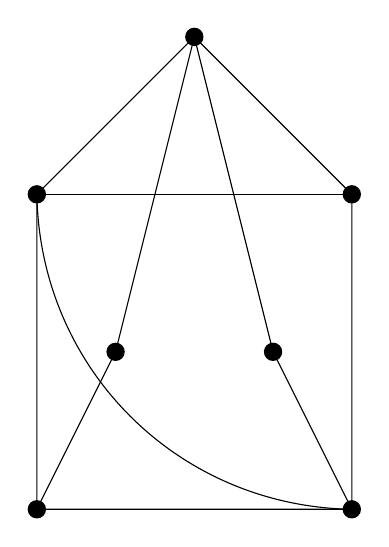
\begin{tikzpicture}
\node[fill=black,  circle, inner sep=0pt,minimum width=0.5mm] (test) at (0,0) {\textbullet};
\node[fill=black,  circle, inner sep=0pt,minimum width=0.5mm] (test) at (0,4) {\textbullet};
\node[fill=black,  circle, inner sep=0pt,minimum width=0.5mm] (test) at (4,4) {\textbullet};
\node[fill=black,  circle, inner sep=0pt,minimum width=0.5mm] (test) at (4,0) {\textbullet};
\node[fill=black,  circle, inner sep=0pt,minimum width=0.5mm] (test) at (2,6) {\textbullet};
\node[fill=black,  circle, inner sep=0pt,minimum width=0.5mm] (test) at (1,2) {\textbullet};
\node[fill=black,  circle, inner sep=0pt,minimum width=0.5mm] (test) at (3,2) {\textbullet};

\draw (0,0)--(0,4)--(2,6)--(4,4)--(4,0)--cycle;
\draw (0,4)--(4,4);
\draw (0,0)--(1,2)--(2,6);
\draw (4,0)--(3,2)--(2,6);
\draw (0,4) to[out=-89, in=179] (4,0);
\end{tikzpicture}

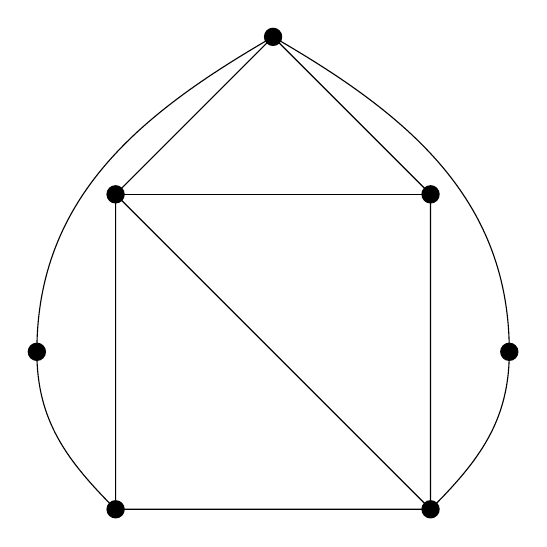
\begin{tikzpicture}
\node[fill=black,  circle, inner sep=0pt,minimum width=0.5mm] (test) at (1,0) {\textbullet};
\node[fill=black,  circle, inner sep=0pt,minimum width=0.5mm] (test) at (1,4) {\textbullet};
\node[fill=black,  circle, inner sep=0pt,minimum width=0.5mm] (test) at (5,4) {\textbullet};
\node[fill=black,  circle, inner sep=0pt,minimum width=0.5mm] (test) at (5,0) {\textbullet};
\node[fill=black,  circle, inner sep=0pt,minimum width=0.5mm] (test) at (3,6) {\textbullet};
\node[fill=black,  circle, inner sep=0pt,minimum width=0.5mm] (test) at (0,2) {\textbullet};
\node[fill=black,  circle, inner sep=0pt,minimum width=0.5mm] (test) at (6,2) {\textbullet};
\draw (1,0)--(1,4)--(3,6)--(5,4)--(5,0)--cycle;
\draw (1,4)--(5,4);
\draw (1,0) to[out=135,in=-90](0,2)to[out=90,in=-150](3,6);
\draw (5,0) to[out=45,in=-90](6,2)to[out=90,in=-30](3,6);
\draw (1,4)--(5,0);
\end{tikzpicture}
\end{center}




\subsection{Graphes planaires}
\begin{mytheo} [Fáry]
Tout graphe planaire simple peut être représenté en n'utilisant que des arêtes droites.
%no proof ?
\end{mytheo}



\begin{mytheo}
Le graphe complet $K_5$ à cinq noeuds n'est pas planaire.

\begin{proof}

Représentons $K_5$ dans le plan. Soit l'ensemble de ses noeuds $\{v_1, v_2, v_3, v_4, v_5\}$.\\
$v_1, v_2$ et $v_3$ forment un triangle. Où placer $v_4$?

\begin{center}
\begin{tikzpicture}
\node[circle] (v1)[draw=black] at (0,0) {v1};
\node[circle] (v2)[draw=black] at (7,0) {v2};
\node[circle] (v3)[draw=black] at (2,5) {v3};
\draw (v1)--(v2)--(v3)--(v1);
\end{tikzpicture}
\end{center}


\begin{enumerate}
\item A l'intérieur du triangle formé par $v_1, v_2$ et $v_3$ ?\\
\begin{center}
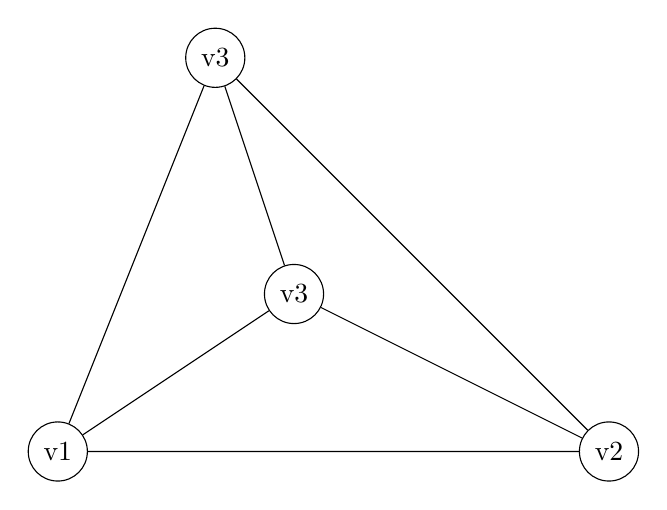
\begin{tikzpicture}
\node[circle] (v1)[draw=black] at (0,0) {v1};
\node[circle] (v2)[draw=black] at (7,0) {v2};
\node[circle] (v3)[draw=black] at (2,5) {v3};
\node[circle] (v4)[draw=black] at (3,2) {v3};
\draw (v1)--(v2)--(v3)--(v1);
\draw (v4)--(v1);
\draw (v4)--(v2);
\draw (v4)--(v3);
\end{tikzpicture}
\end{center}
%\includegraphics[scale=0.4]{t2}\\
Où placer $v_5$?
\begin{enumerate}
\item A l'intérieur du triangle formé par $v_1, v_3$ et $v_4$ ? Le graphe ne serait plus planaire puisqu'il faudrait couper le triangle $v_1, v_3$ et $v_4$ pour relier $v_5$ à $v_2$.\\
\begin{center}
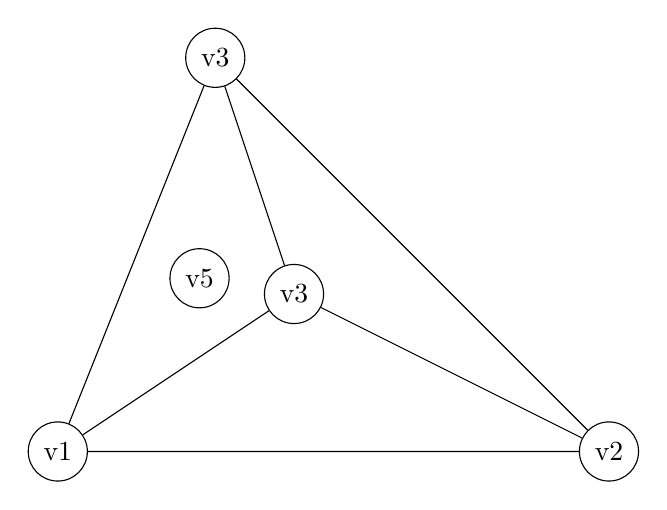
\begin{tikzpicture}
\node[circle] (v1)[draw=black] at (0,0) {v1};
\node[circle] (v2)[draw=black] at (7,0) {v2};
\node[circle] (v3)[draw=black] at (2,5) {v3};
\node[circle] (v4)[draw=black] at (3,2) {v3};
\node[circle] (v5)[draw=black] at (1.8,2.2) {v5};
\draw (v1)--(v2)--(v3)--(v1);
\draw (v4)--(v1);
\draw (v4)--(v2);
\draw (v4)--(v3);
\end{tikzpicture}
\end{center}
%\includegraphics[scale=0.4]{t3}
\item A l'intérieur de $v_1$, $v_2$, $v_4$ ou de $v_2$, $v_3$, $v_4$ ? Idem.
\item A l'extérieur de $v_1$, $v_2$, $v_3$? \\
\begin{center}
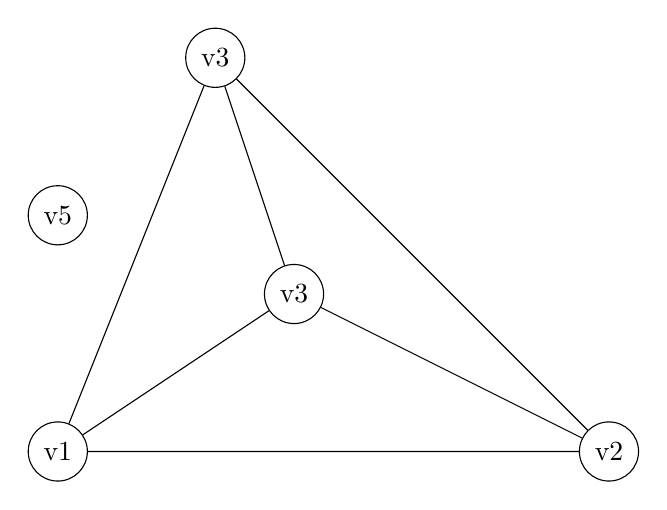
\begin{tikzpicture}
\node[circle] (v1)[draw=black] at (0,0) {v1};
\node[circle] (v2)[draw=black] at (7,0) {v2};
\node[circle] (v3)[draw=black] at (2,5) {v3};
\node[circle] (v4)[draw=black] at (3,2) {v3};
\node[circle] (v5)[draw=black] at (0,3) {v5};
\draw (v1)--(v2)--(v3)--(v1);
\draw (v4)--(v1);
\draw (v4)--(v2);
\draw (v4)--(v3);
\end{tikzpicture}
\end{center}
%\includegraphics[scale=0.4]{t4}\\
\end{enumerate}
\item A l'extérieur de $v_1, v_2$, $v_3$ ? En applicant le même type d'énumération qu'au point précédent, on trouve qu'il n'y a aucune manière de représenter $K_5$ dans le plan de manière à ce qu'il soit planaire.
\end{enumerate}
\end{proof}
\end{mytheo}



\begin{mytheo}
Le graphe complet biparti $K_{3,3}$ à $3+3$ noeuds n'est pas planaire.
\begin{proof}
Preuve \addTODO
\end{proof}
\end{mytheo}



\begin{mytheo} [Kuratowski]
  Un graphe est non planaire si et seulement s'il contient comme sous-graphe $K_5$ ou $K_{3,3}$ ou une subdivision de ceux-ci.
  \begin{proof}
    Preuve \addTODO
  \end{proof}
\end{mytheo}


\index{subdivision}
\begin{mydef}
  Une \emph{subdivision} (remplacement de chaque arête par un chemin) d'un graphe non planaire est non-planaire, et un sous-graphe d'un graphe planaire est planaire.
\end{mydef}

\index{face}
\index{face!face extérieure}
\index{face!face intérieure}
\begin{mydef}
  Un graphe planaire (dans une représentation sans croisement) découpe le plan en plusieurs régions connexes (au sens géométrique). Ces régions sont appelées \emph{faces}. Il y a une et une seule face non bornée, nommée \emph{face extérieure}, les autres faces sont \emph{intérieures}.
\end{mydef}

\index{face!bord d'une face}
\index{face!face incidente}
\index{face!degré d'une face}
\begin{mydef}
  On identifie le \emph{bord d'une face} au parcours fermé qui longe la face. Le bord parcourt chaque arête une ou deux fois. 
  Une face est \emph{incidente} aux arêtes et sommets qui sont sur son bord.
  Le \emph{degré d'une face} est la longueur du bord, donc le nombre d'arêtes incidentes (comptées une ou deux fois).
\end{mydef}
\begin{myexem}
  Exemple \addTODO
\end{myexem}

\index{dual}
\begin{mydef}
  Etant donné un graphe planaire $G$ (dans une représentation sans croisement), construisons $G^*$ , graphe dont les sommets sont les faces de $G$, reliés si et seulement si les faces correspondantes ont dans $G$ une arête en commun. Ce graphe $G^*$ est le \emph{dual} de $G$ (dans cette représentation).
\end{mydef}
\begin{myexem}

\noindent
\textit{Exemple} : \\
\begin{center}
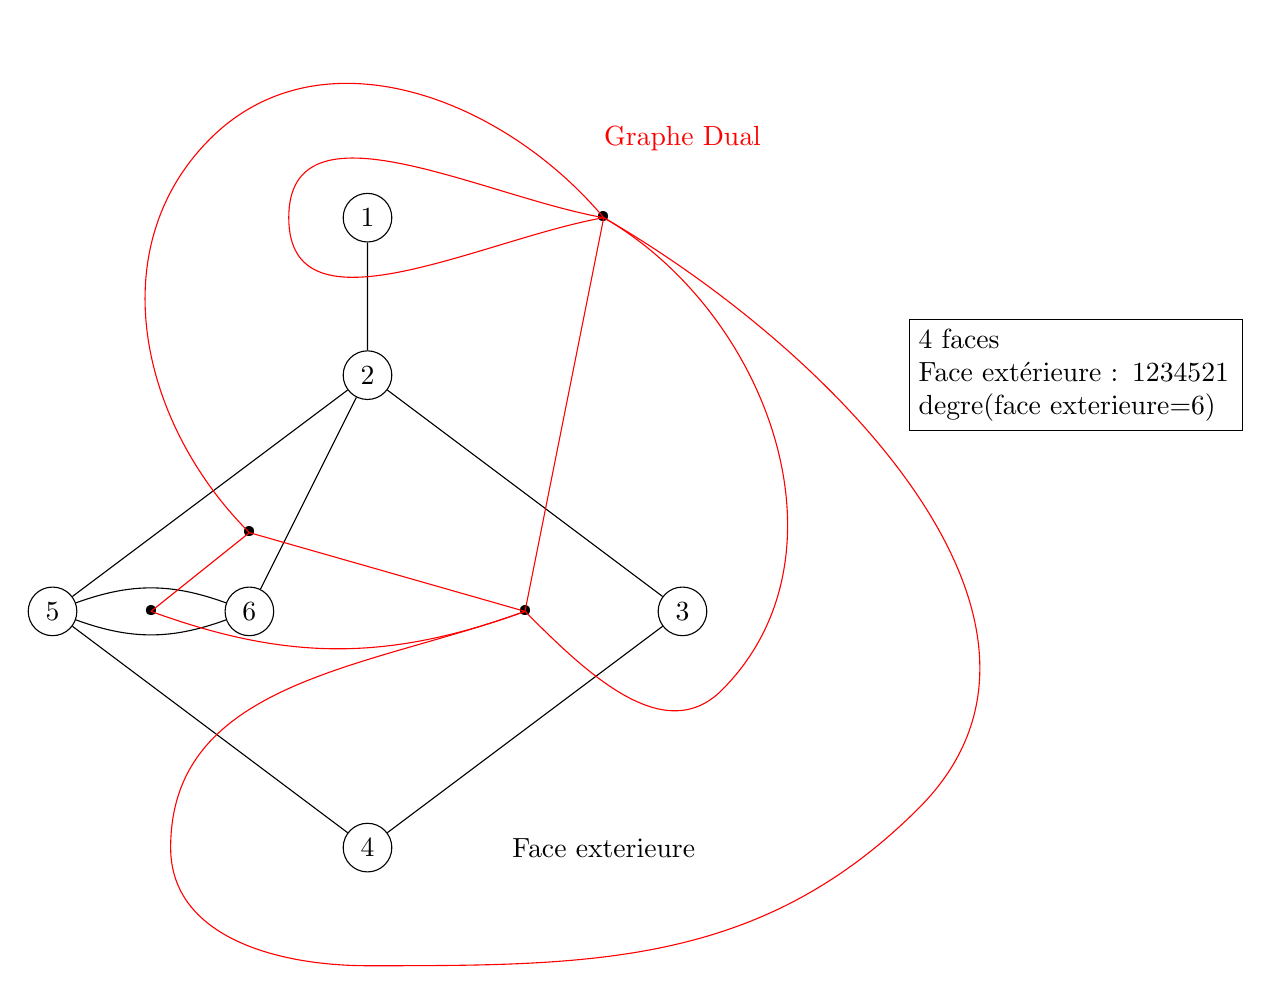
\begin{tikzpicture}
%Premier graphe
\node[circle](N1)[draw=black] at (4,10) {1};
\node[circle](N2)[draw=black] at (4,8) {2};
\node[circle](N3)[draw=black] at (8,5) {3};
\node[circle](N4)[draw=black] at (4,2) {4};
\node[circle](N5)[draw=black] at (0,5) {5};
\node[circle](N6)[draw=black] at (2.5,5){6};

\draw (N1)--(N2)--(N3)--(N4)--(N5)--(N2);
\draw (N5)to[out=20,in=160](N6)to[out=-160,in=-20](N5);
\draw (N6)--(N2);

%Second graphe
\node (NN7) at (1.25,5) {\textbullet};
\node (NN8) at (2.5,6) {\textbullet};
\node (NN9) at (7,10) {\textbullet};
\node (NN10) at (6,5) {\textbullet};
\node [red] (test) at (8,11){Graphe Dual};
\node [black] (test) at  (7,2){Face exterieure};
\node [draw,text width =4cm] (test) at (13,8) 
{4 faces\\
Face extérieure : 1234521\\
degre(face exterieure=6)};

\coordinate (N7) at (1.25,5);
\coordinate (N8) at (2.5,6);
\coordinate (N9) at (7,10);
\coordinate (N10) at (6,5);

\draw[red] (N7) to[out=-20,in=-160](N10)--(N8)--(N7);
\draw[red] (N10)to[out=-160,in=90](1.5,2)to[out=-90,in=-180](4,0.5)to[out=0,in=-135](11,2.5)to[out=45,in=-30](N9)to[out=130,in=45](2,11)to[out=-135,in=135](N8);
\draw[red] (N10)to[out=-45,in=-135](8.5,4)to[out=45,in=-30](N9);
\draw[red] (N10)--(N9);
\draw[red] (N9) to[out=170,in=90](3,10)to[out=-90,in=-170](N9);

\end{tikzpicture}
\end{center}
\end{myexem}


\begin{mytheo}
  La somme des degrés des faces est deux fois le nombre d'arêtes.
  \begin{proof}
    Preuve \addTODO
  \end{proof}
\end{mytheo}

\begin{mytheo}
  Un graphe est planaire si et seulement si il est représentable sur la sphère sans croisement d'arêtes.
  \begin{proof}
    Preuve \addTODO
  \end{proof}
\end{mytheo}

%TODO END


\subsection{Formule d'Euler}
\begin{mytheo} [Formule d'Euler]
  Dans un graphe planaire connexe à $n$ sommets, $e$ arêtes et $f$ faces:\\
  $n−e+f =2$
  \begin{proof}
    On démontre cette égalité par récurrence sur sur le nombre d'arêtes. 
    	
    Si le graphe est sans cycle $\Rightarrow$ la face extérieure est la seule face. Le graphe est donc un arbre et on a donc 
    $$|arêtes|= |sommets|-1,$$ 
    $$|sommets| - |aretes| + |faces|= 2.$$	
    
  Si il existe un cycle, il y a donc deux faces adjacentes. En supprimant une arête entre les deux faces, les deux faces deviennent une seule et le nombre de faces moins le nombre d'arêtes reste constant. Par hypothèse de récurrence on a donc que  
  $$|sommets| - |aretes| + |faces|$$ 
  n'est pas modifié et vaut 2.
   
  \end{proof}
\end{mytheo}

\begin{mytheo}
  \label{theo:threensix}
  Dans tout graphe planaire \emph{simple} à $n \geq 3$ sommets et $e$ arêtes,
  $e \leq 3n - 6$.
  \begin{proof}
    Si il n'y a qu'une seule face, évident. 
    
    Si il y a au moins une face, le bord de la face a au moins 3 arêtes (vu que la plus petite face possible est un triangle et que c'est une graphe simple). On a donc deg(face)$\geq 3$. Et donc $$\sum \text{deg(face)} \geq 3 |faces| .$$
Or    $$\sum \text{deg(face)} = 2 |aretes|.$$
Et donc 
 \begin{equation} \label{ineg6}
 \frac{2}{3} |aretes| \geq |faces|.
\end{equation} 
    En injectant \ref{ineg6} dans la formule d'Euler, le résultat est démontré.   
  \end{proof}
\end{mytheo}

\begin{mytheo}
  Pour tout graphe planaire \emph{simple}, il y a un noeud de degré $\leq 5$.
  \begin{proof}
    On va montrer que le degré moyen est $< 6$.
    Ce qu'il voudra dire qu'il existe un noeud de degré $\leq 5$.
    \begin{align*}
      \deg_{\mathrm{avg}} & = \frac{\sum_{v\in V} \deg(v)}{|V|}\\
                          & = \frac{2|E|}{|V|}.
    \end{align*}
    Considérons 2 cas
    \begin{itemize}
      \item Si $|V| < 3$, l'énoncé est trivial car dans un graphe simple,
        pour tout $v \in V$, $\deg(v) \leq |V|-1$ du coup
        $\deg(v) \leq |V| - 1 < 2 \leq 5$ pour tout $v$.
      \item
        Comme notre graphe est simple,
        on peut utiliser le théorème~\ref{theo:threensix},
        on a donc $|E| \leq 3|V| - 6$.
        Dès lors
        \begin{align*}
          \deg_{\mathrm{avg}} & \leq 2\frac{3|V|-6}{|V|}\\
                              & = 6 - \frac{12}{|V|} < 6.
        \end{align*}
    \end{itemize}
  \end{proof}
\end{mytheo}

\begin{mycorr}
  $K_5$ est non planaire.
  \begin{proof}
    $K_5$ a 5 noeuds et 10 arêtes.
    Par le théorème~\ref{theo:threensix}, $|E| \leq 3|V| - 6$.
    Il faut donc que $10 \leq 3 \cdot 5 - 6 = 9$, ce qui est faux.
    Le graphe est par conséquent non planaire.
  \end{proof}
\end{mycorr}

\begin{mycorr}
  $K_{3,3}$ est non planaire.
  \begin{proof}
    $K_{3,3}$ a 6 noeuds et 9 arêtes.
    C'est un graphe biparti donc les cycles sont de longueur pair de plus il est simple donc tous les cycles ont une longueur $\geq 4$.
    Donc toutes les faces ont un degré $\geq 4$.
    On a alors $\sum_{f \in F} \deg(f) \geq 4|F|$ et par le théorème des poignées de main dual, $\sum_{f \in F} \deg(f) = 2|E| = 18$.
    Donc $|F| \leq \frac{18}{4} = 4.5$.

    Par la formule d'Euler, il faut que
    $|F| - |E| + |V| = 2$.
    Or $|F| - |E| + |V| \leq 4.5 - 9 + 6 = 1.5$.
    $K_{3,3}$ ne peut donc pas être planaire.
  \end{proof}
\end{mycorr}

\subsection{Les cinq solides platoniciens}
\index{solide platonicien}
\begin{mydef}
  Un \emph{solide platonicien} est un polyèdre convexe régulier.
  C'est-à-dire que toutes les faces, sommets et arêtes sont identiques à une rotation près.
\end{mydef}

\begin{mytheo}
  Il y a 5 solides platoniciens.
  \begin{proof}
    Les polyèdres convexes correspondent à des graphes planaires, via projection.
    Le fait qu'ils soient platoniciens nous dit que chaque noeud est de même degré $p$ et que chaque face est de même degré $q$.
    \begin{center}
      \begin{tabular}{ll}
        La formule d'Euler & $|F| - |E| + |V| = 2$\\
        Poignées de main & $p|V| = 2|E|$\\
        Poignées de main dual & $q|F| = 2|E|$
      \end{tabular}
    \end{center}
    Donc
    \begin{align*}
      \frac{2}{q}|E| - |E| + \frac{2}{p} |E| & = 2\\
      \frac{2}{q} - 1 + \frac{2}{p} & = \frac{2}{|E|} > 0\\
      \frac{1}{q} + \frac{1}{p} & > \frac{1}{2}.
    \end{align*}
    On sait donc que soit $p$, soit $q$ est $< 4$ (ou les deux).
    Or $p \geq 3$ et $q \geq 3$ (par géométrie, graphes planaires simple de dual simple).
    Les possibilités sont
    \begin{center}
      \begin{tabular}{|c|c|c|c|c|c|}
        \hline
        $p$ & $q$ & $|V|$ & $|F|$ & $|E|$ & Polyèdre\\
        \hline
         3  &  3  &   4   &   4   &   6   & Tétraèdre\\
         3  &  4  &   8   &   6   &  12   & Cube\\
         4  &  3  &   6   &   8   &  12   & Octaèdre\\
         3  &  5  &  20   &  12   &  30   & Dodécaèdre\\
         5  &  3  &  12   &  20   &  30   & Icosaèdre\\
        \hline
      \end{tabular}
    \end{center}
  \end{proof}
\end{mytheo}

\begin{mytheo} [Kempe]
  Tout graphe planaire possède un coloriage propre à cinq couleurs.
  ``Toute carte peut être coloriée avec 5 couleurs''.\\
  Nombre chromatique $\chi$ (graphe planaire) $\leq 5$.
  \begin{proof}
    Par récurrence: ``on enlève un noeud, on colorie par hyp. de récurrence, on remet le noeud.''
    On peut supposer le graphe \emph{simple} (car arêtesmultiples n'affectent pas $\chi$).
    Il existe un noeud $u$ de degré $\leq 5$.
    On enlève $u$, on a encore un graphe planaire, on le colorie.
    On rétablit $u$:
    \begin{itemize}
      \item si $\deg(u) < 5$: facile, on utilise une couleur non utilisée par les voisins pour $u$.
      \item Si $\deg(u) = 5$: Si ces 5 voisins utilisent $< 5$ couleurs: facile aussi.
        Si 5 couleurs utilisées $c_1, c_2, c_3, c_4, c_5$.
        Regardons $v_1$ et $v_3$. Si $v_1$ et $v_3$ sont sur des composantes connexes différentes: on échange $c_1$ et $c_3$ sur
        la composante connexe ($c_1-c_3$) de $v_3$, et on colorie $u$ en $c_1$ (sur le graphe des noeuds de couleur $c_1$ et $c_3$.
        Si $v_1$ et $v_3$ sont dans la même composante connexe ($c_1-c_3$):
        Maintenant $v_2$ et $v_4$ sont dans des composantes connexes
        différentes (dans le graphe de couleurs $c_2-c_4$).
        Même raisonnement: échanger $c_2$ et $c_4$ sur composante connexe ($v_2$).
    \end{itemize}
  \end{proof}
\end{mytheo}

\begin{mytheo} [Appel, Haken]
  Tout graphe planaire possède un coloriage propre à quatre couleurs.
  \begin{proof}
    Preuve \addTODO
  \end{proof}
\end{mytheo}
